\begin{frame}{Candidate descriptor leaders: potential and capacity}
\centering
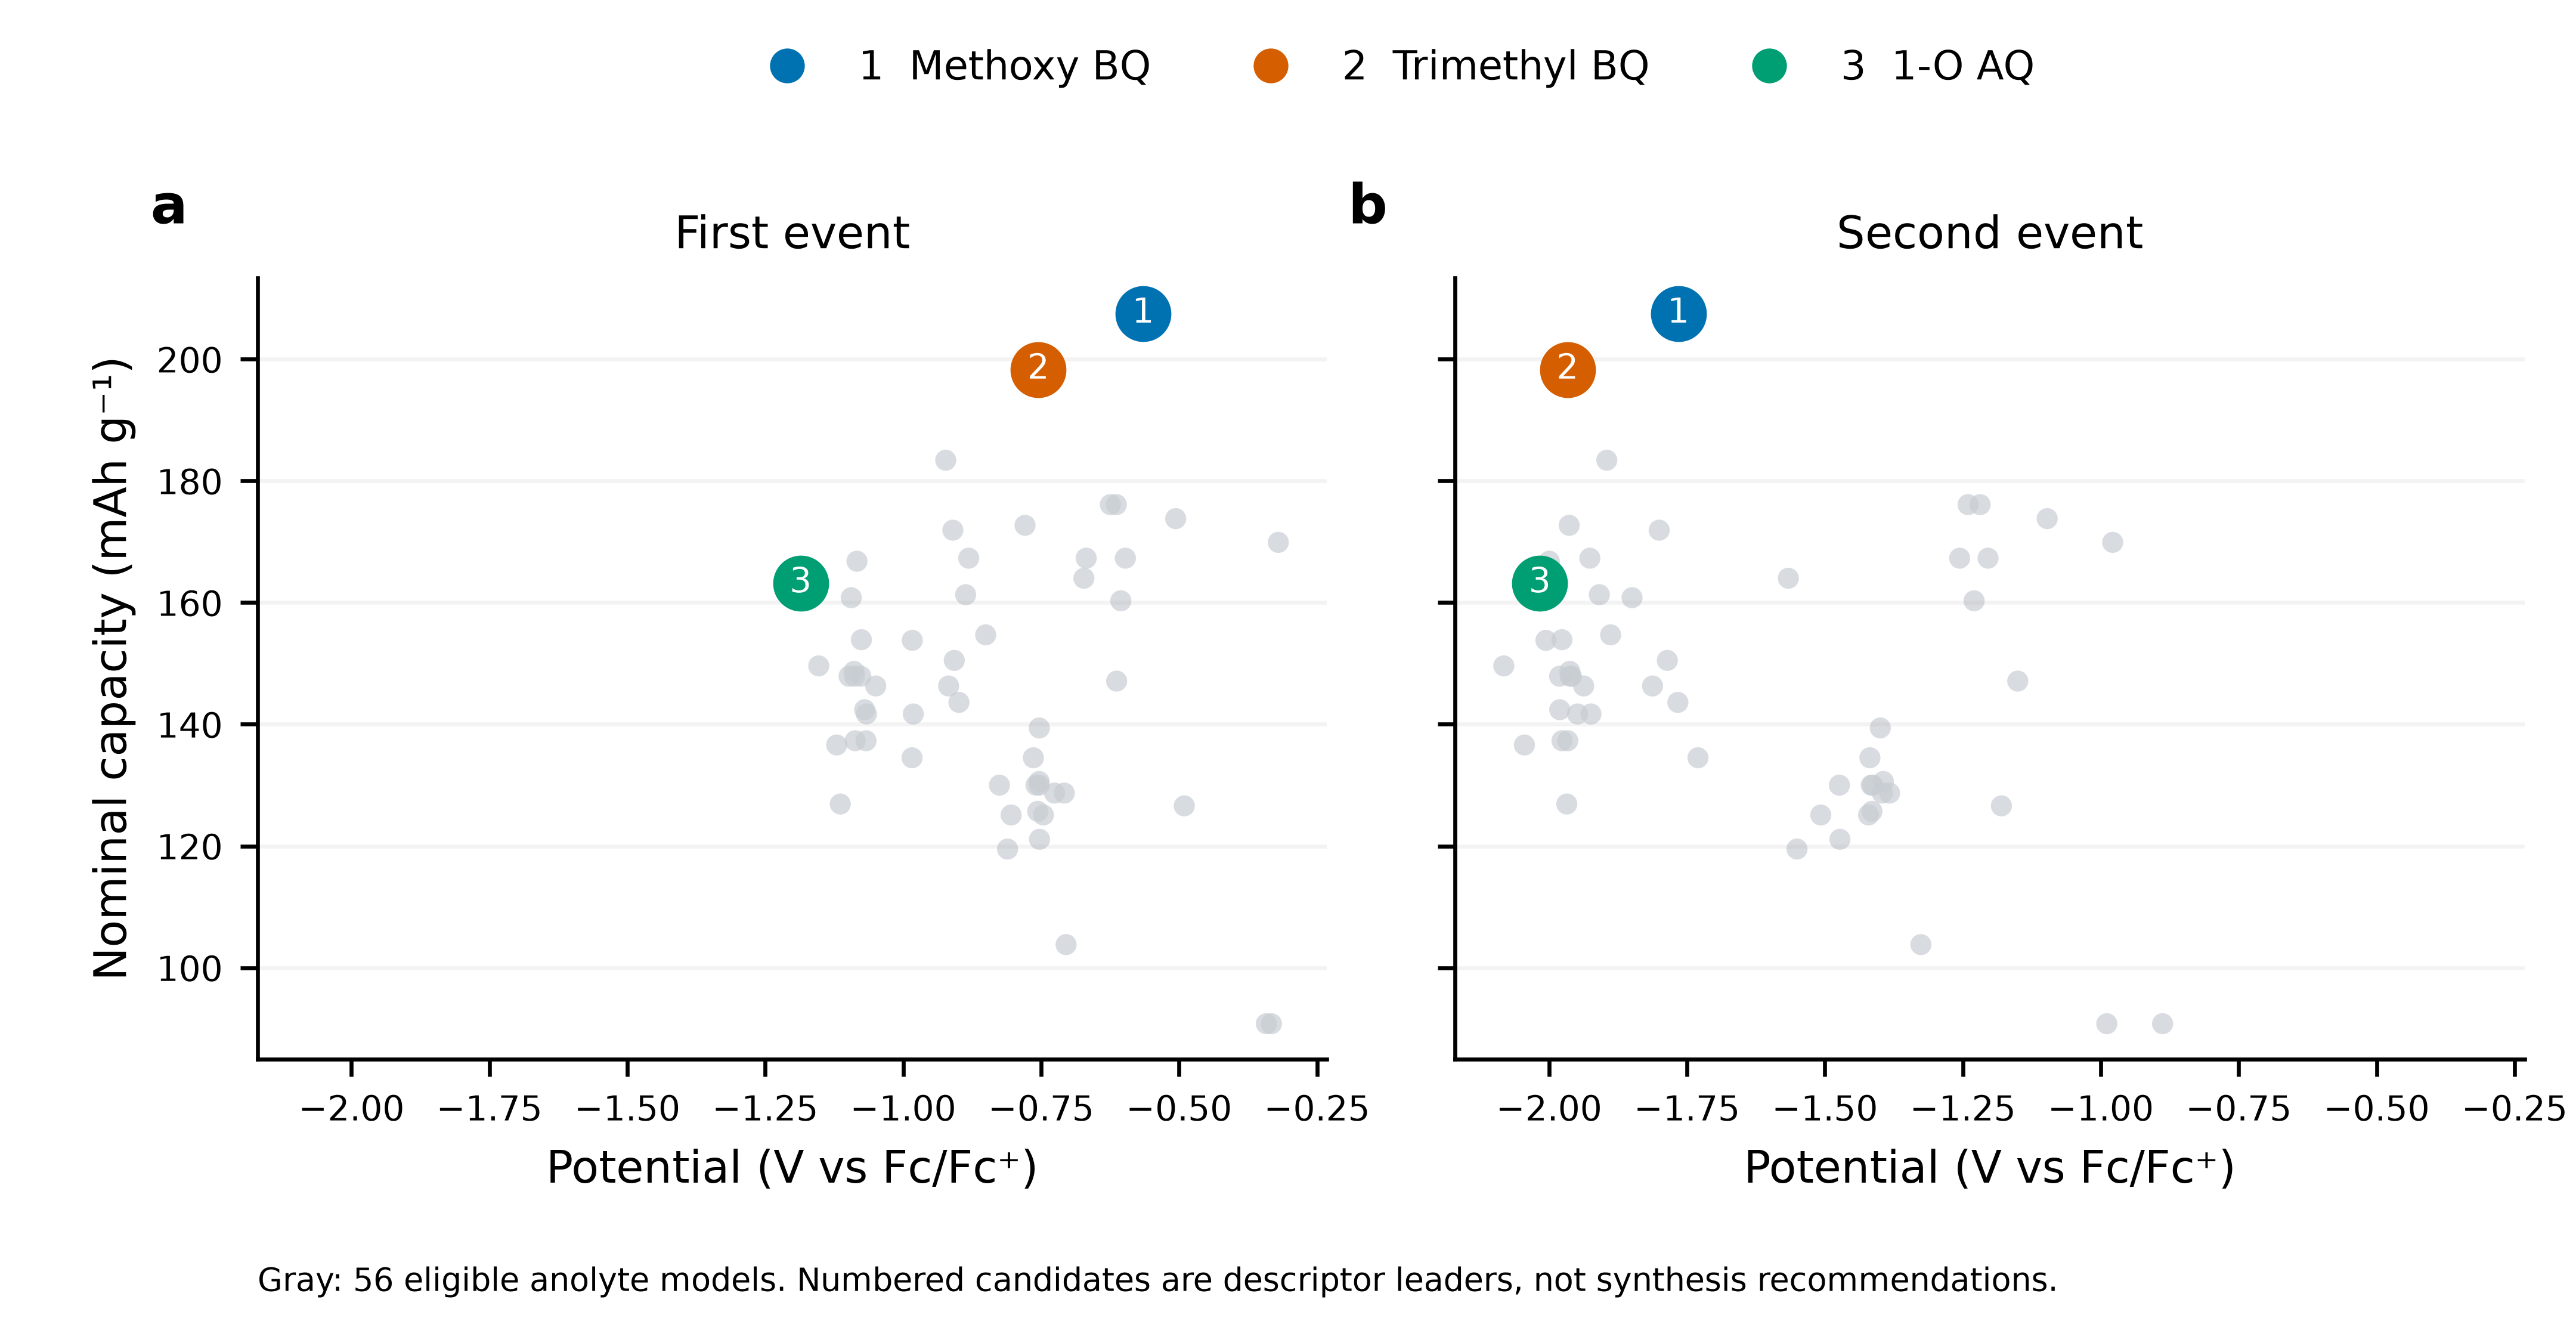
\includegraphics[width=.97\linewidth,height=.72\textheight,keepaspectratio]{../results/candidates/figures/plots/redox_capacity.png}
\par\smallskip\raggedright\scriptsize Numbers identify anolyte descriptor leaders on a partial potential--capacity front. Kinetics and polymer validation remain pending.
\vfill\tiny Audited model snapshot: 2026-10-23T05:33:27.705929-05:00.
\end{frame}
\begin{frame}{Synthesis accessibility is a separate consideration}
\centering
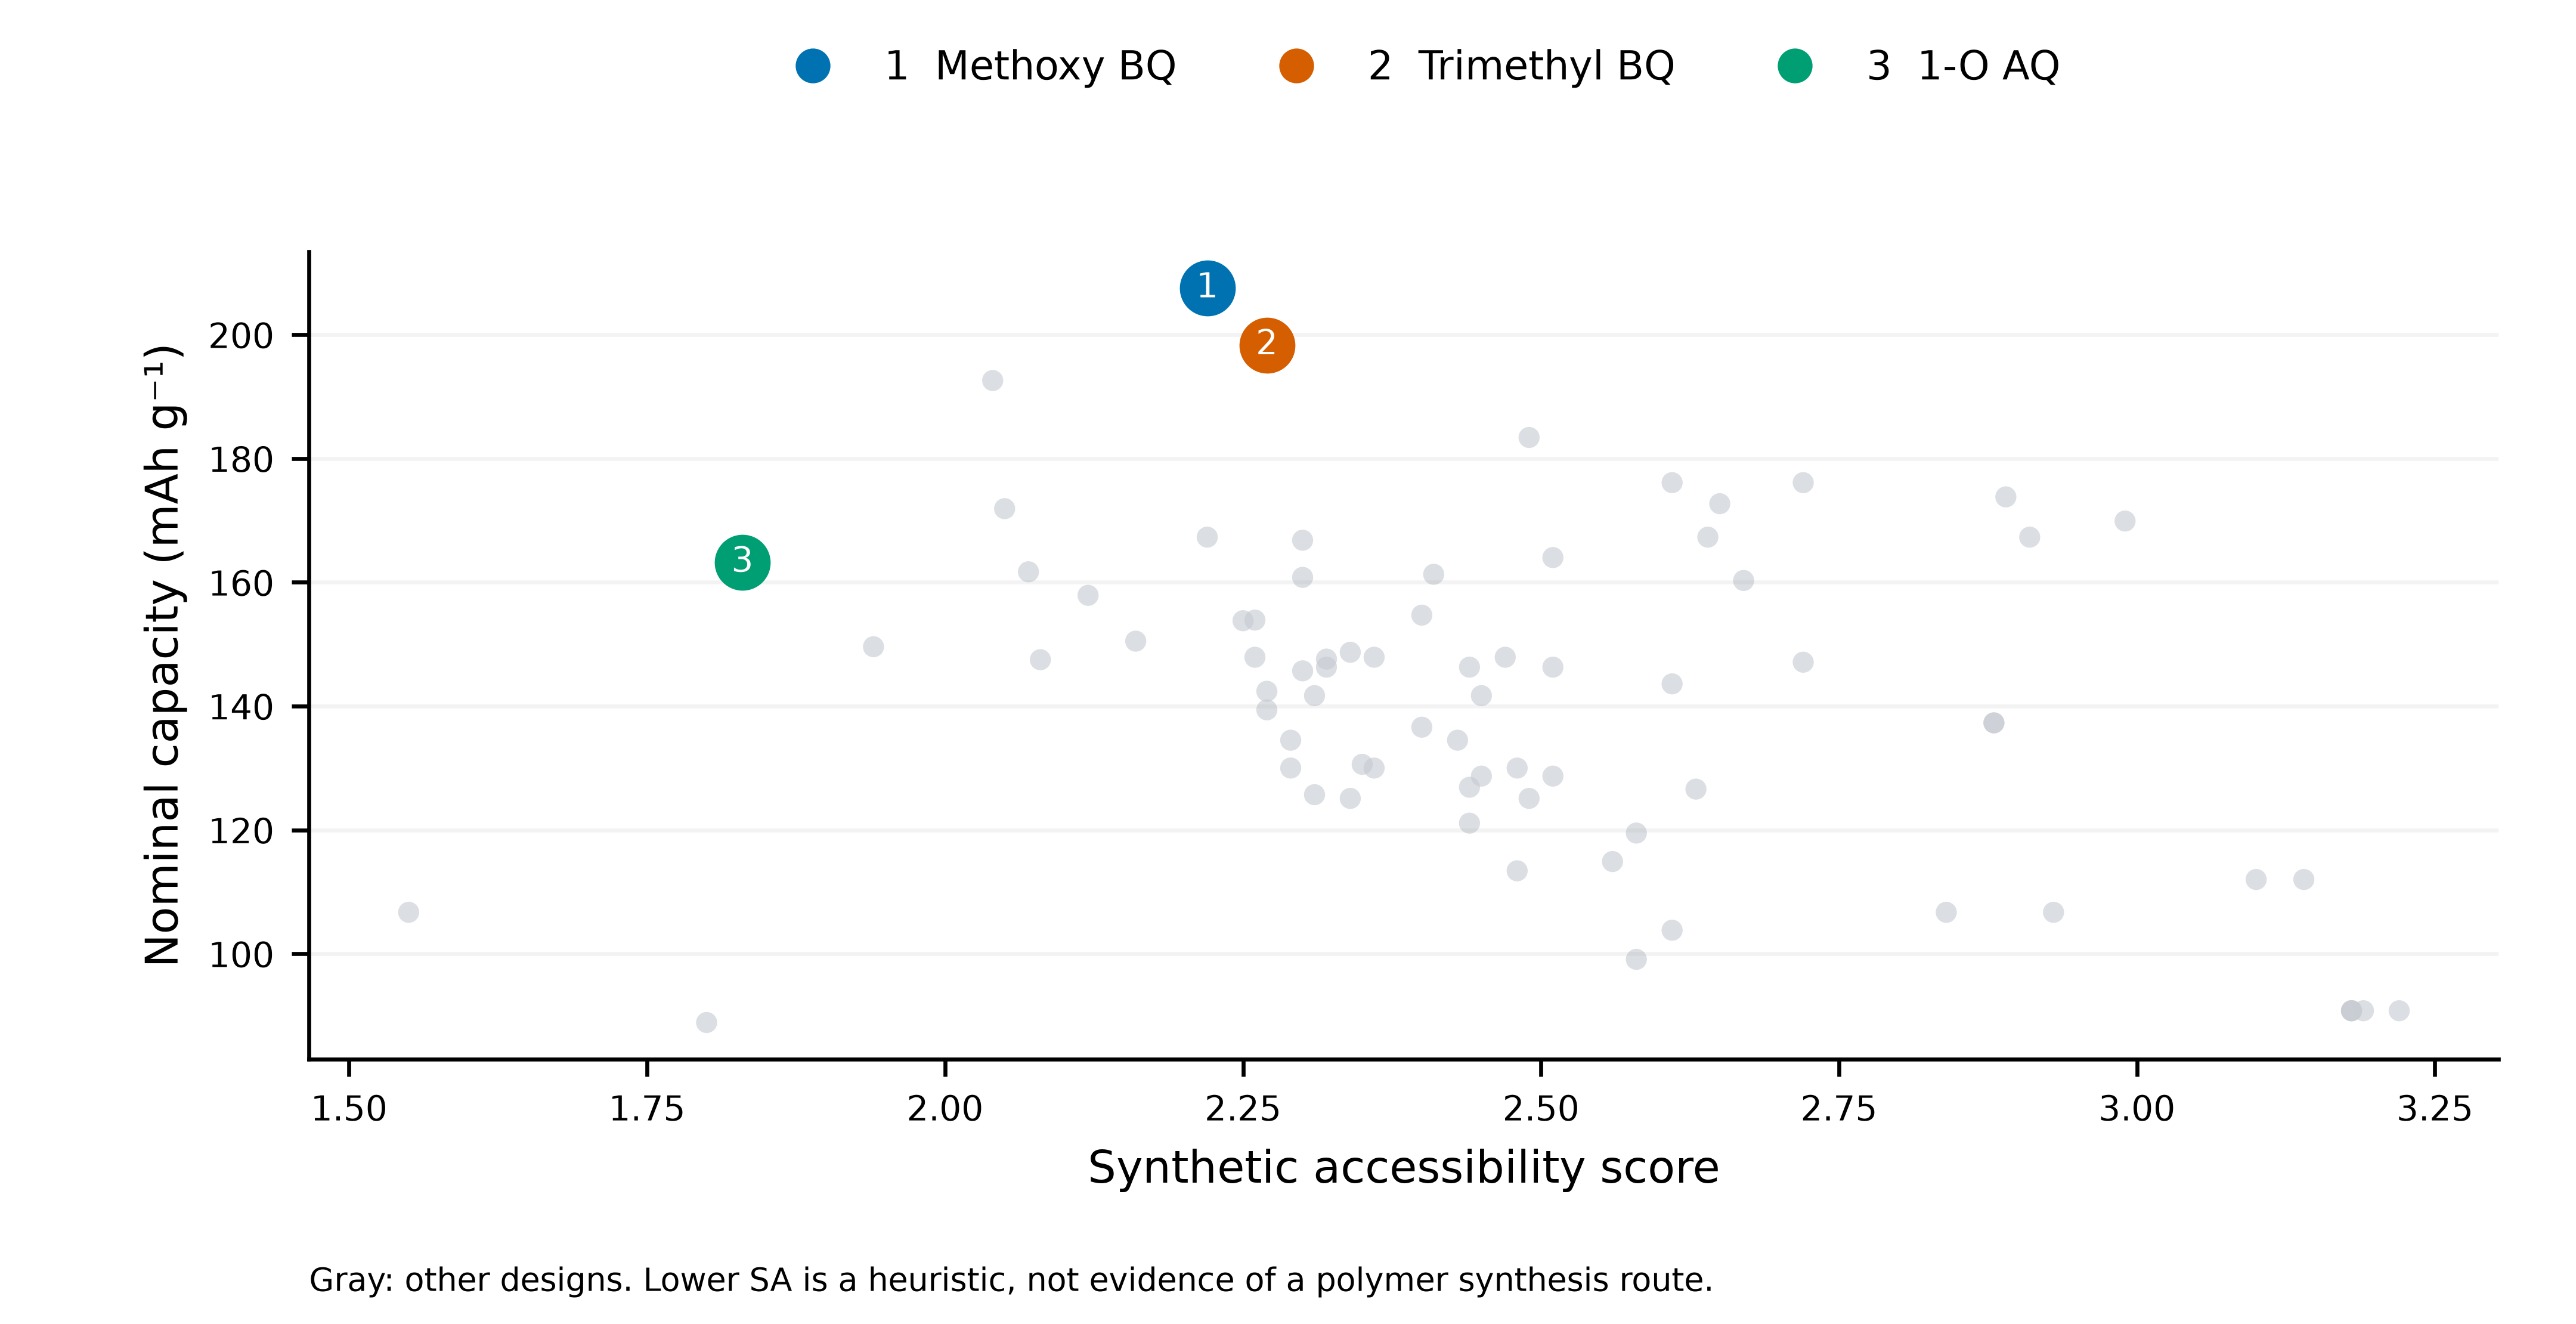
\includegraphics[width=.97\linewidth,height=.72\textheight,keepaspectratio]{../results/candidates/figures/plots/synthesis_tradeoff.png}
\par\smallskip\raggedright\scriptsize SA is a heuristic annotation. The local methylbenzyl caps model graft sites; precursor chemistry, loading and accessibility require separate review.
\vfill\tiny Audited model snapshot: 2026-10-23T05:33:27.705929-05:00.
\end{frame}
\begin{frame}{New candidate contrasts against matched controls}
\centering
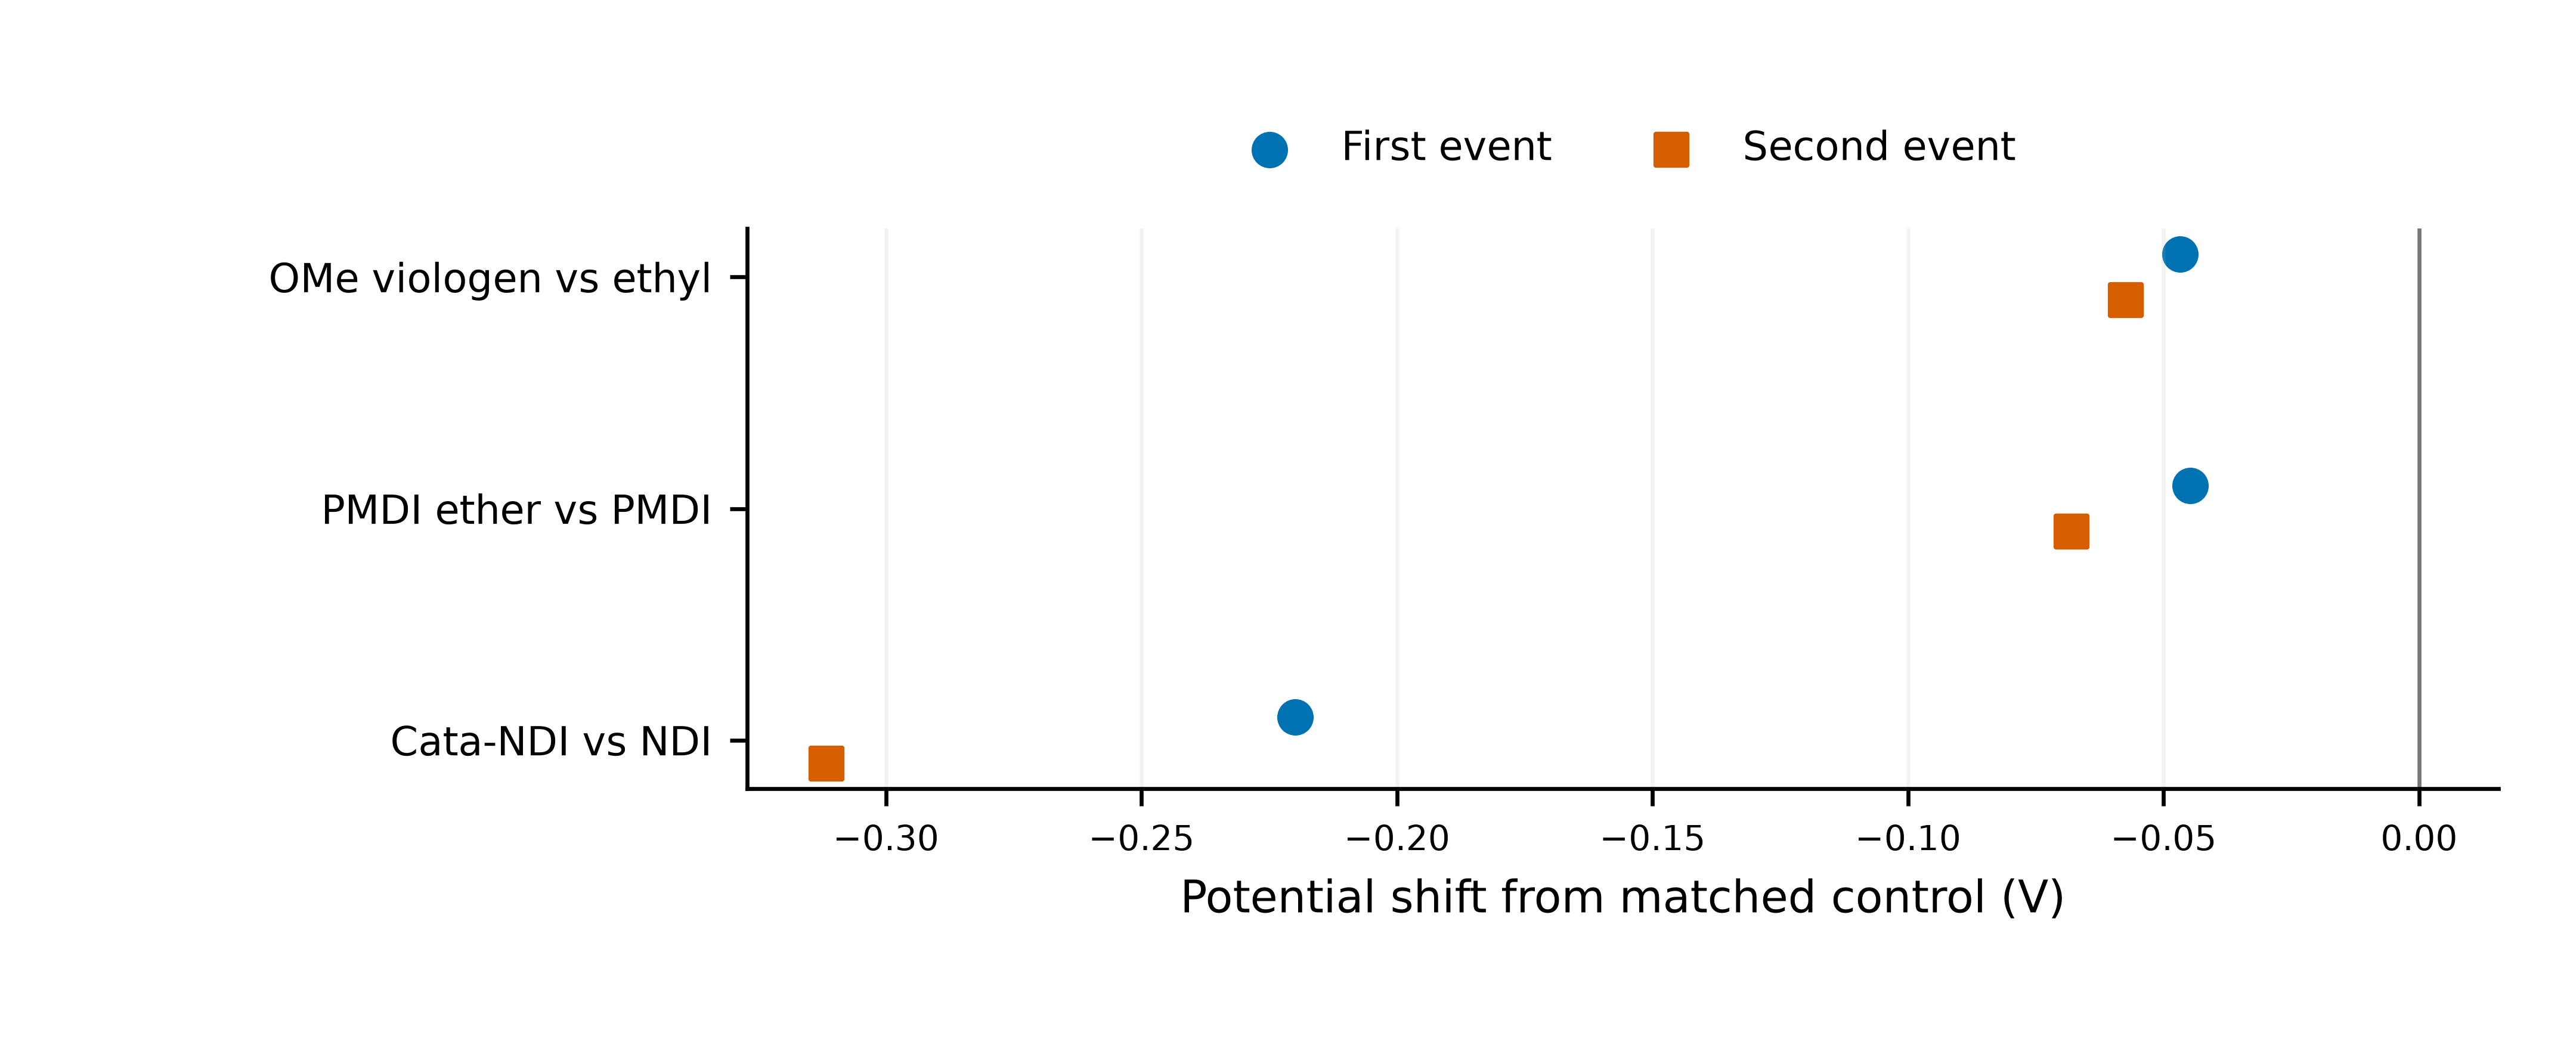
\includegraphics[width=.97\linewidth,height=.72\textheight,keepaspectratio]{../results/candidates/figures/plots/new_candidate_shifts.png}
\par\smallskip\raggedright\scriptsize One contrast per core with the strongest potential decrease shared by both events. A shift does not establish polymer performance.
\vfill\tiny Audited model snapshot: 2026-10-23T05:33:27.705929-05:00.
\end{frame}
\begin{frame}{Molecular structures: computed graft-site models}
\centering
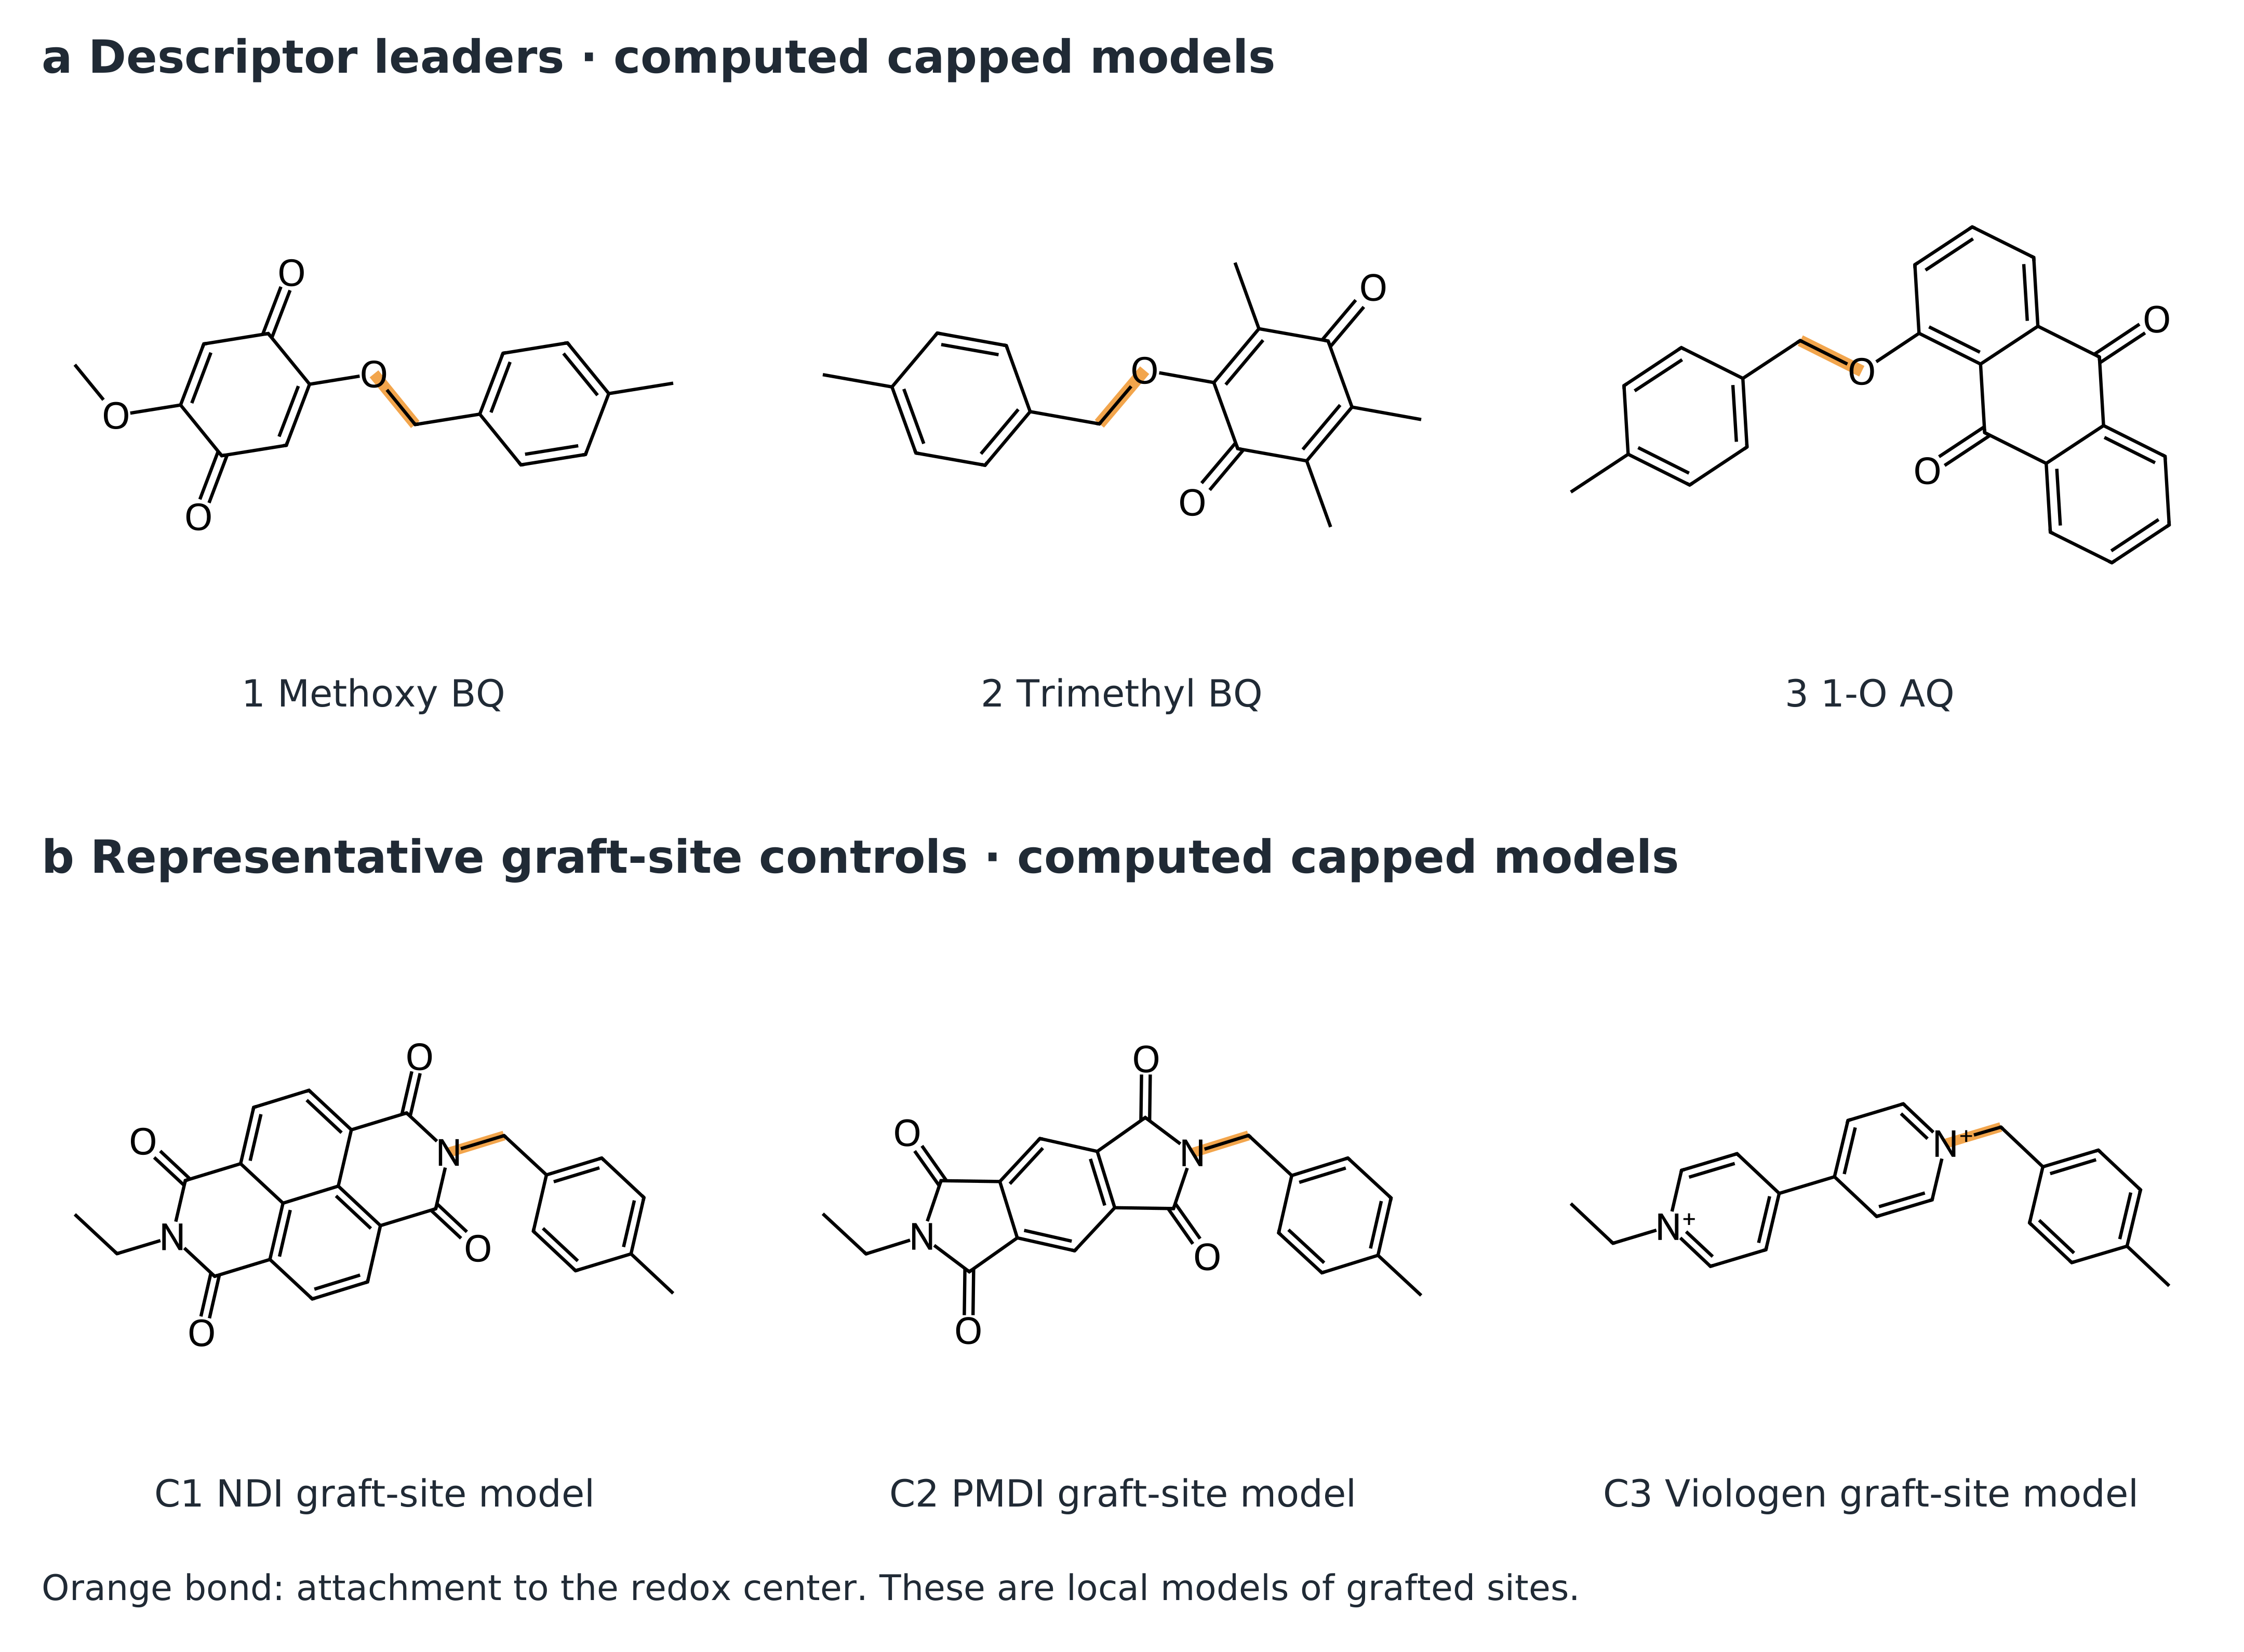
\includegraphics[width=.97\linewidth,height=.72\textheight,keepaspectratio]{../results/candidates/figures/structures/candidate_structures.png}
\par\smallskip\raggedright\scriptsize Top: computed capped-model descriptor leaders. Bottom: representative capped graft-site controls. Orange marks attachment.
\vfill\tiny Audited model snapshot: 2026-10-23T05:33:27.705929-05:00.
\end{frame}
